\documentclass[]{scrartcl}
\usepackage[spanish]{babel}

\decimalpoint
%opening
\usepackage{xcolor}
\usepackage{mathtools}
\usepackage{graphicx}
\usepackage{enumitem}
\usepackage{hyperref}
\newcommand{\tt}[1]{\texttt{#1}}

\newcommand{\that}[0]{\texttt{THAT~}}

\usepackage{siunitx}
\sisetup{output-decimal-marker = {.}}

\title{Práctica 2 de control: computación analógica y control PI}
\author{Leonardo Bermeo}

\begin{document}
	
	\maketitle
%
%
%
%\section{Generador de onda cuadrada\label{sec:cuadrada}}
%El computador analógico \tt{THAT} tiene una señal que indica cuando los integradores de cómputo son \emph{reseteados} periodicamente al elegir uno de los modos repetitivos (\tt{REP} o \tt{REPF}). Dicha señal está en la salida \tt{TR}. Vamos a usar esa señal para generar una onda cuadrada que nos permita obtener la respuesta al escalón para los sistemas analógicos que implementaremos.
%\begin{enumerate}[label=\alph*)]
%	\item Conecte el cable RCA blanco a las señales \texttt{TR} (trigger) y \texttt{U} del \tt{THAT} como se muestra en la figura~\ref{fig:jackrca}. 
%%
%\begin{figure}[h!]
%	\centering
%	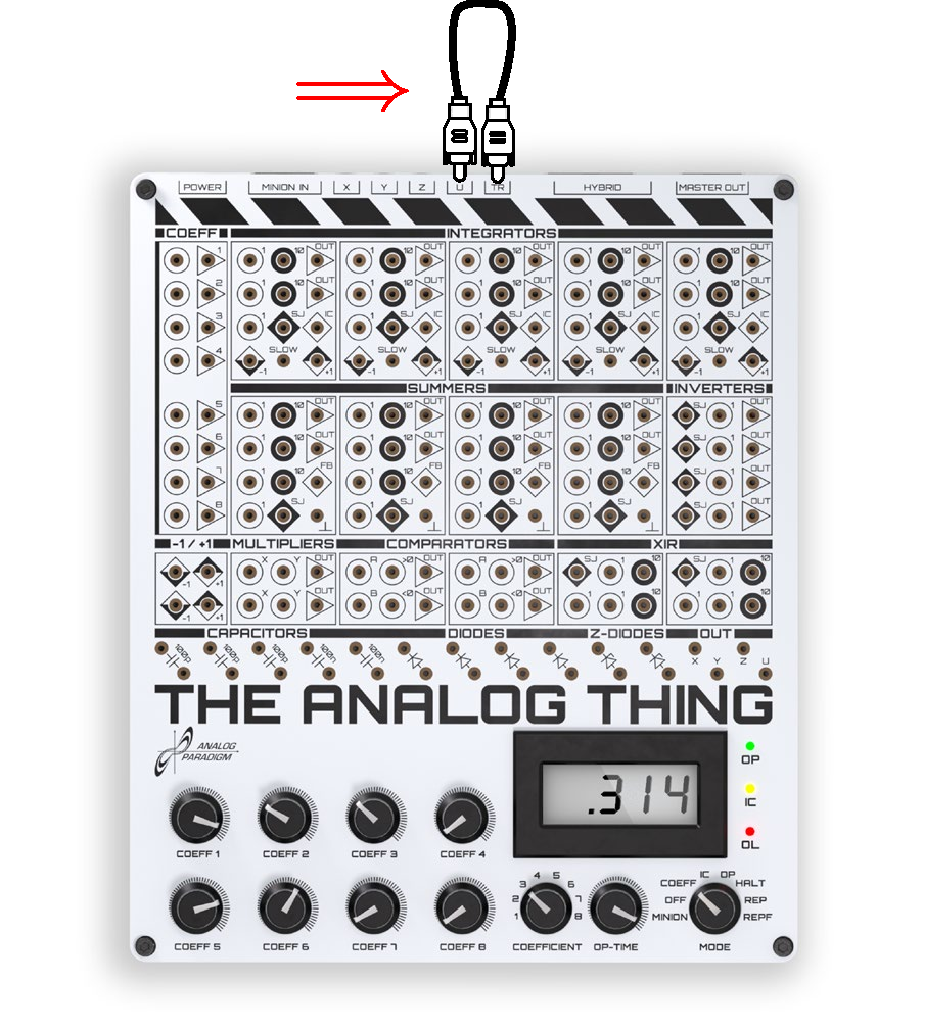
\includegraphics[width=0.5\linewidth]{figuras/jackrca}
%	\caption{Conector RCA}
%	\label{fig:jackrca}
%\end{figure}
%\newpage
%\item  Realice cuidadodamente las conexiones que se ilustran en la figura \ref{fig:onda_cuad}
%%
%\begin{figure}[h!]
%	\centering
%	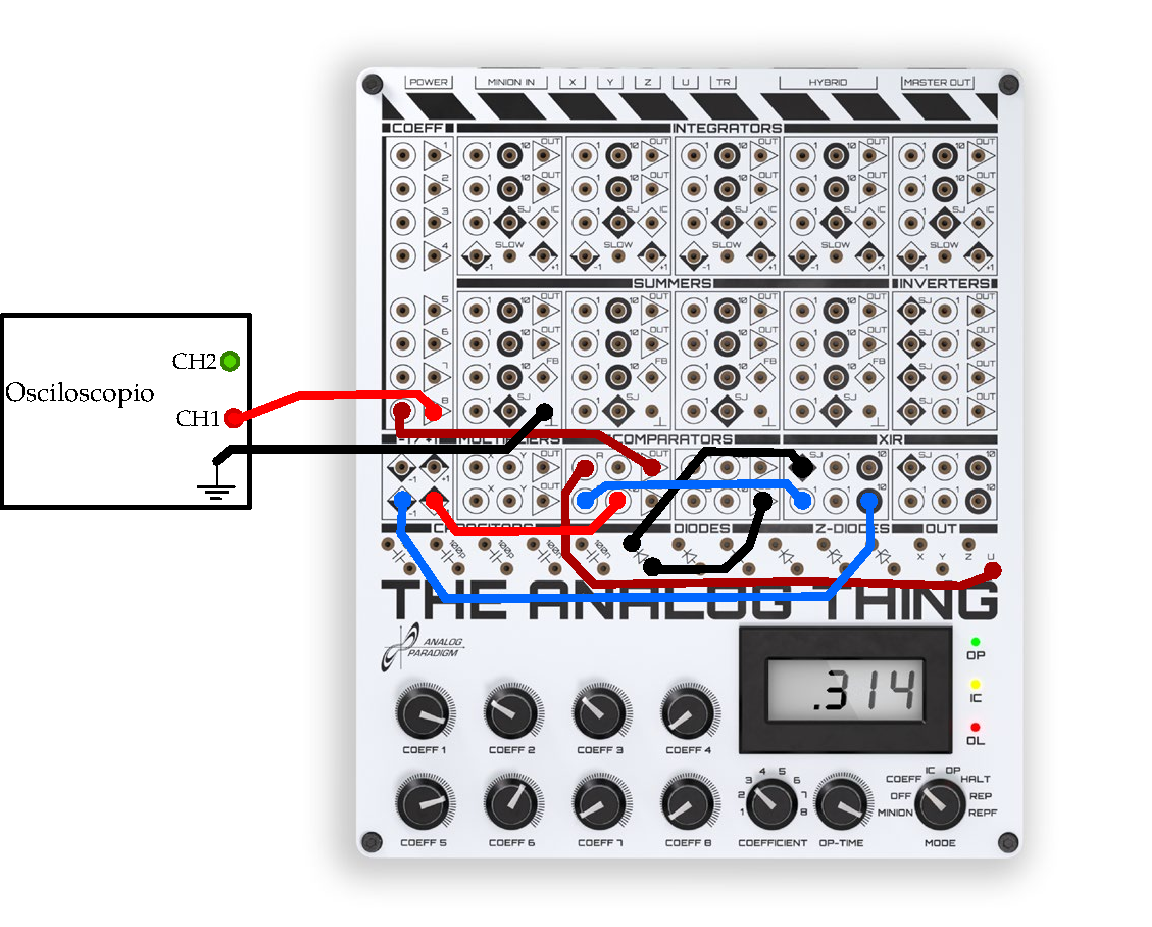
\includegraphics[width=0.8\linewidth]{figuras/onda_cuadrada1}
%	\caption{Conexiones para la onda cuadrada}
%	\label{fig:onda_cuad}
%\end{figure}
%%\item Conecte los cables RCA desde las señales \texttt{X} e \texttt{Y} del \tt{THAT} a los canales 1 y 2 del osciloscopio como se muestra, usando los conversores de RCA a BNC suministrados. 
%%%
%%\begin{figure}[h!]
%%	\centering
%%	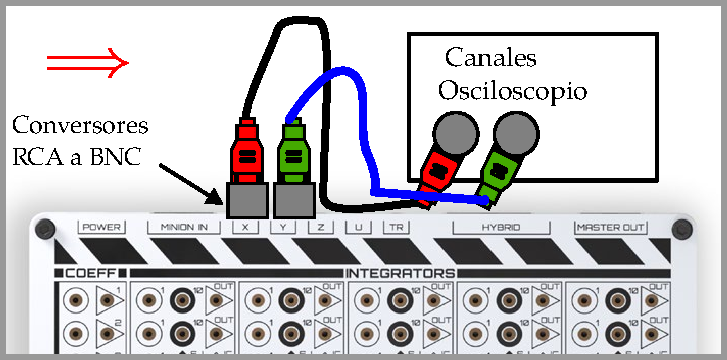
\includegraphics[width=0.7\linewidth]{figuras/canales_osc}
%%	\caption{Conexiones para el osciloscopio}
%%	\label{fig:canales_osc}
%%\end{figure}
%
%\item Conecte el cargador USB-C a la entrada \texttt{POWER} del \tt{THAT}.
%
%\item Ajuste el selector  \texttt{MODE} en \texttt{REPF}  (repetitive fast),  es decir, con repetición rápida del reset de los integradores . Ajuste el tiempo entre cada reset de los integradores con el potenciométro de \texttt{OP-TIME} al máximo, como se ilustra en la figura~\ref{fig:botones}.  
%%
%\begin{figure}[h!]
%	\centering
%	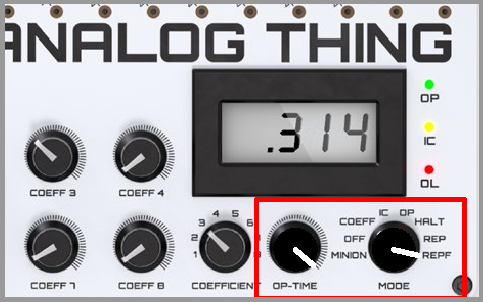
\includegraphics[width=0.5\linewidth]{figuras/botones_repf}
%	\caption{Ajuste de los botones}
%	\label{fig:botones}
%\end{figure}
%
%
%\item Sincronice adecuadamente el canal 1 del osciloscopio. Debe estar visualizando una señal cuadrada como la mostrada en la figura~\ref{fig:senal_osc}. El osciloscopio debe estar en acople CC en toda esta práctica.
%%
%\begin{figure}[h!]
%	\centering
%	
\includegraphics[width=0.6\linewidth]{figuras/osc_cuadrada1}
%	\caption{Señal cuadrada}
%	\label{fig:senal_osc}
%\end{figure}
%\newpage
%\item Verifique que el potenciómetro \tt{COEFF 8}  ajusta la amplitud del escalón la onda cuadrada. Ajuste la amplitud en 5V,  aproximadamente. 
% %
% \begin{figure}[h!]
% 	\centering
% 	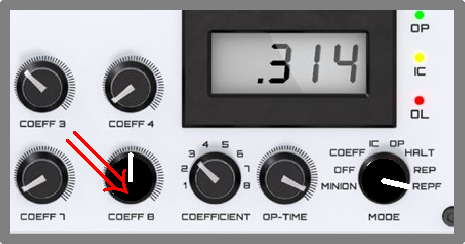
\includegraphics[width=0.5\linewidth]{figuras/amplitude_cuadrada}
% 	\caption{Botón de control de Amplitud}
% 	\label{fig:boton_amplitud}
% \end{figure}
%
%\end{enumerate}
%

\section{Bloques de computación analógica básica}

El \tt{THAT} tiene varios bloques de computación analógica (multiplicadores, comparadores). Vamos a usar los siguientes bloques en esta práctica, junto con las convenciones mostradas en la figura~\ref{fig:tabla_analog}.
%
\begin{figure}[h!]
	\centering
	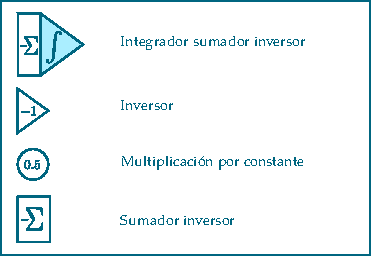
\includegraphics[width=0.6\linewidth]{figuras/tabla_analog}
	\caption{Bloques analógicos.}
	\label{fig:tabla_analog}
\end{figure}

\section{Sistema de Segundo orden}

Ahora si vamos a usar el \tt{THAT} para implementar sistemas como los vistos en la teoria. Comenzaremos por un sistema de segundo orden con función de transferencia dada por:

\begin{equation}
	H(s)=\dfrac{1}{s^2+bs + 1}, b>0.
\end{equation}

Donde el parámetro $b$ es una variable que ajustaremos con el computador analógico para lograr diferentes comportamientos. \\

Como hemos visto, la representación en variables de estado de este sistema está dada por:
\begin{align*}
	\begin{bmatrix}
		\dot{x_1} \\
		\dot{x_2}
	\end{bmatrix}&=
	\begin{bmatrix}
		-b &-1  \\
		1 & 0
	\end{bmatrix}	
	\begin{bmatrix}
		 x_1 \\
		 x_2
	\end{bmatrix} + 
		\begin{bmatrix}
		1 \\
		0
	\end{bmatrix} u 	\\
	y &= \begin{bmatrix}
		0 & 1
	\end{bmatrix}
		\begin{bmatrix}
		x_1 \\
		x_2
	\end{bmatrix}
\end{align*}
Es decir, las ecuaciones de estado para este sistema las podemos escribir como:
\begin{align}
	\dot{x_1}&= -b\,x_1 - x_2\nonumber\\
	\dot{x_2}&= x_1\nonumber\\
	y&=x_2\label{equ:est2orden}z
\end{align}



\subsection{Implementación del sistema de segundo orden}

Con base en los bloques de computación analógica en la figura~\ref{fig:tabla_analog} vamos a implementar las ecuaciones de estado en \eqref{equ:est2orden}. Estas ecuaciones se implementan de acuerdo al  diagrama de computación analógica de la figura~\ref{fig:analog2order}:
 %
\begin{figure}[h!]
	\centering
	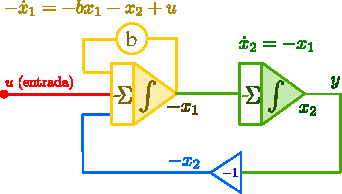
\includegraphics[width=0.6\linewidth]{figuras/analog2order}
	\caption{Implementación analógica del sistema de segundo orden.}
	\label{fig:analog2order}
\end{figure}

Note que las variables de estado a la salida de los integradores siempre salen invertidas. Por ello, si suponemos que a la entrada del segundo integrador está $-x_1$ su salida debe ser $x_2$.

\newpage

\subsubsection{Pasos de Implementación en el THAT}
\begin{enumerate}[label=\alph*)]
	\item Identifique cada uno de los componentes del diagrama de la figura~\ref{fig:analog2orderthat}. Se puede guiar por la salidas de los integradores. Las lineas del diagrama de computación analógica están con los mismos colores sugeridos para las conexiones entre elementos del \tt{THAT}. Note que a la izquierda está la multiplicación por el coeficiente $b$ y a la derecha el inversor azul. 
 %
\begin{figure}[h!]
	\centering
	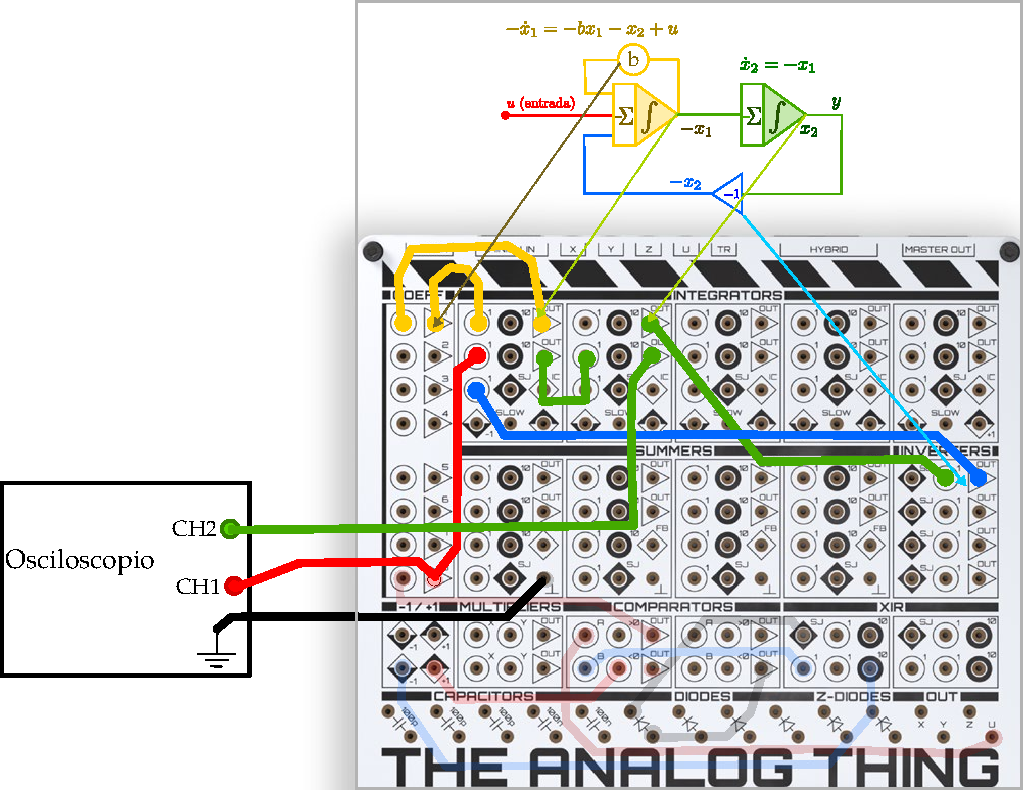
\includegraphics[width=0.9\linewidth]{figuras/analog2orderthat}
	\caption{Implementación analógica del sistema de segundo orden.}
	\label{fig:analog2orderthat}
\end{figure}
	\item Implementar cuidadosamente el diagrama de computador analógico de la figura~\ref{fig:analog2orderthat}. Note que no es necesario (ni deseable) conectar la tierra del canal 2.
	\item Ponga la perilla \tt{MODE} del \tt{THAT} en \tt{COEFF} y ajuste el potenciómetro del coeficiente $b$ en 1. Regrese la perilla al modo \tt{REPF}.
	
	\newpage
	\item Sincronice los dos canales del osciloscopio para ver la respuesta al escalón del sistema de segundo orden implementado. Use como fuente de sincronia el escalón (canal 1) y ajuste el trigger apropiadamente para obtener una imagen fija. Debe estar obteniendo una respuesta similar a esta:
	%
	\begin{figure}[h!]
		\centering
		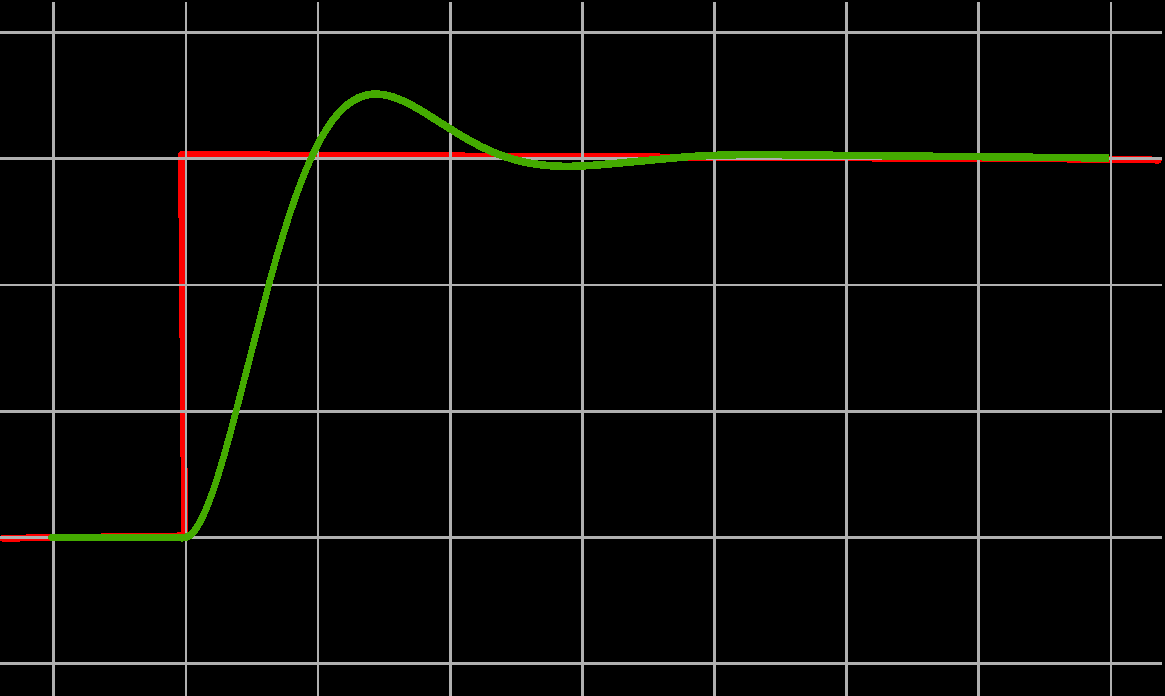
\includegraphics[width=0.6\linewidth]{figuras/osc}
		\caption{Señal del sistema de segundo orden}
		\label{fig:senal2orden}
	\end{figure}
	\item Varie suavemente el valor del potenciométro de  $b$ y observe lo que ocurre. Discuta con su compañero.
	\item Obtenga la respuesta para valores de $b$ = 0, 0.25, 0.5, 1. No es necesario ser tan preciso. Haga con su compañero un bosquejo aproximado de la localización de los polos en el plano complejo para estos valores de $b$. Indique si hay casos en que el sistema es inestable.

	\item Acceda a \href{https://colab.research.google.com/drive/1b7orSCMo12l76fKedXTSs88f4nAhV3Ly?usp=sharing}{este notebook de colab}, ejecute cada una de las celdas, compare con su bosquejo y los resultados que obtuvo.
	\item ¿Qué valor mínimo de $b$ necesitamos para obtener un sistema amortiguado (sin oscilaciones, con polos reales)? 
	\item ¿Cómo podemos obtenerlo en el \tt{THAT}? Revise la sección~\ref{sec:coefmay} y produzca un sistema amortiguado, sin oscilaciones. 
	
\end{enumerate}

\subsubsection{Sistema inestable}

Ahora vamos a implementar el mismo sistema de segundo orden pero con un pequeño cambio. La función de transferencia que vamos a implementar  es ahora la siguiente:
\begin{equation}
	H(s)=\dfrac{1}{s^2-bs+1}, b>0.	
	\label{equ:inestable}
\end{equation}

Note para implementar la ecuación~\eqref{equ:inestable} solo es necesario colocar un inversor para $b$ como se ilustra a continuación:
 %
\begin{figure}[h!]
	\centering
	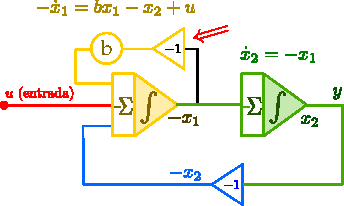
\includegraphics[width=0.5\linewidth]{figuras/analog2orderinest}
	\caption{Implementación analógica del sistema de segundo orden con coeficiente  negativo.}
	\label{fig:2orderinestable}
\end{figure}

\begin{enumerate}[label=\alph*)]
	\item Discuta con su compañero de trabajo si el sistema de la ecuación~\eqref{equ:inestable} es estable o inestable.

	\item Realice esta modificación en el  \tt{THAT} para implementar el sistema de la figura~\ref{fig:2orderinestable}.
	 %
	\begin{figure}[h!]
		\centering
		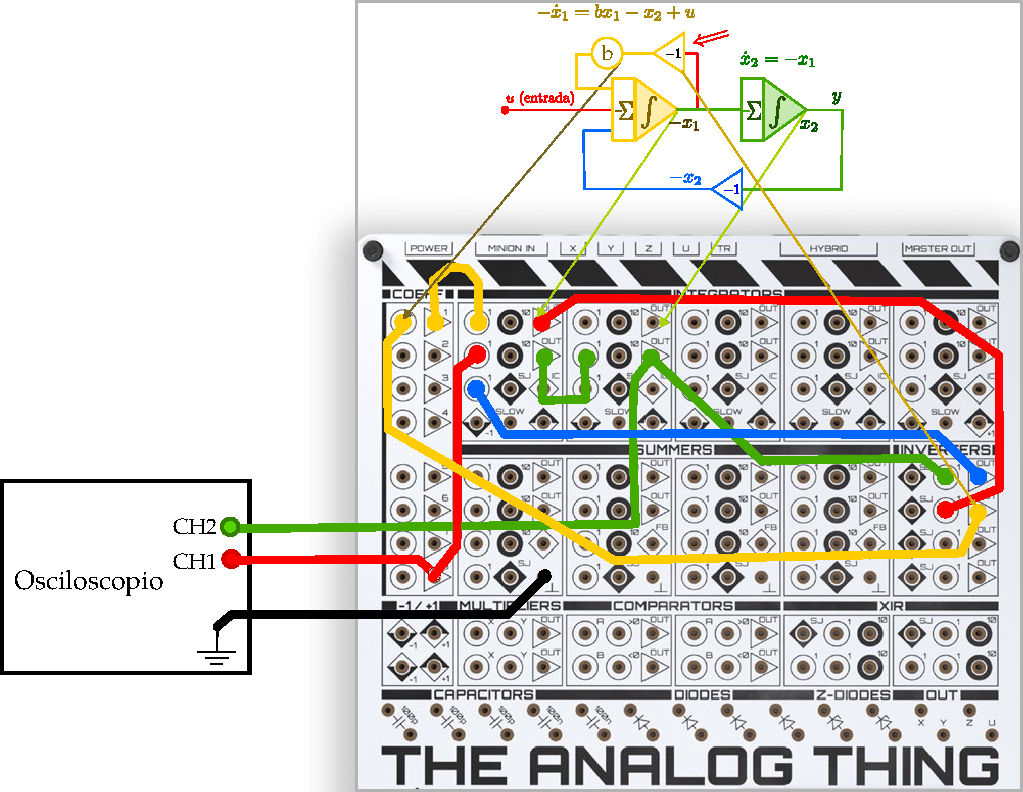
\includegraphics[width=0.9\linewidth]{figuras/analog2orderthatinest}
		\caption{Implementación analógica del sistema de segundo orden con coeficiente negativo.}
		\label{fig:analog2orderinest}
\end{figure}

\item Ajuste la tensión del escalón de entrada con \tt{COEFF 8} en aproximadamente 1V. Sincronice el osciloscopio con este escalón.
\item Varie suavemente el valor de $b$ y observe lo que ocurre.
\item Discuta lo que ocurre cuando $b=.05$ y cuando $b=0.1$. Haga un bosquejo de la ubicación de los polos del sistema en el plano complejo para estos casos.
\item Discuta sobre la estabilidad de este sistema.
\item Compare sus resultados con los que se obtienen en \href{https://colab.research.google.com/drive/1yLNEhGWMdqoO_5xwOrW4sqK69zA014Ml?usp=sharing}{este colab}
\end{enumerate}

%\section{Sistema de lazo cerrado y test de Rooth-Hurwitz}
\newpage
\section{Filtro analógico de Chebyschev}

\subsection{Especificaciones y diseño}

En esta parte vamos a implementar un filtro analógico con las siguientes especificaciones:

\begin{itemize}
	\item Frecuencia de corte real: $f_{p,real}=100\,\text{Hz}$
	\item Rizado en la banda de paso: $\alpha_P=0.1\,\text{dB}$
	\item Atenuación en la banda de rechazo: $\alpha_S=25\text{dB}$
\end{itemize}

\emph{Nota:} Los condensadores y resistencias del \tt{THAT} no se pueden cambiar. Como el \tt{THAT} tiene resistencias y condensadores en los  integradores con constante de tiempo $RC=1M\Omega \times 1\text{nF} = 0.001s$, asumiremos que la frecuencia angular normalizada  para el \tt{THAT} es de

\[ 1/RC=1/0.01=1000\text{rad/s.}\]

Esto quiere decir que con los coeficientes numéricos que obtendremos para un filtro con frecuencia normalizada en 1, la frecuencia de corte del \tt{THAT} será $\overline{\omega_P}=1000\text{rad/s}$, esto es, $159.15\text{Hz}$. 

Si requerimos un filtro para una frecuencia de $100Hz$, debemos diseñar para la frecuencia

\[\omega_p= \dfrac{2\times \pi \times f_{p,real}}{1000}=  \dfrac{2\times \pi \times 1000}{100}=0.628\, \text{rad/s}\] 


En este \href{https://colab.research.google.com/drive/1FAwNfmSHj2Xydje-8FpgHDbYV_laZE4f?usp=sharing}{notebook de colab} está el diseño del filtro para la frecuencia  $f_{p,real}=100\,\text{Hz}$ requerida.


\subsection{Implementación del filtro analógico}

Una vez diseñado el filtro obtenemos una función de transferencia en secciones de segundo orden dada por:
\begin{equation}
	H(s)= \underbrace{\dfrac{0.128}{s^2 + 0.801\,s + 0.246}}_{H_1(s)} \times \underbrace{\dfrac{1}{s^2 + 0.332\,s + 0.525}}_{H_2(s)} 
	\label{equ:filcheb}          
\end{equation} 
Vamos a escribir el filtro de la ecuación~\eqref{equ:filcheb} de la siguiente forma más general: 
\begin{equation}
	H(s)= \underbrace{\dfrac{b_{0}}{s^2 + a_{11}\,s + a_{01}}}_{H_1(s)} \times \underbrace{\dfrac{1}{s^2 + a_{12}\,s + a_{02}}}_{H_2(s)}
	\label{equ:filchebgen}          
\end{equation} 

La implementación de la función de transferencia $H(s)=H_1(s)\times H_2(s)$ de la ecuación~\eqref{equ:filchebgen} se puede realizar de acuerdo al diagrama de computación analógica mostrado en la figura~\ref{fig:filtrocomp}.
	 %
\begin{figure}[th!]
	\centering
	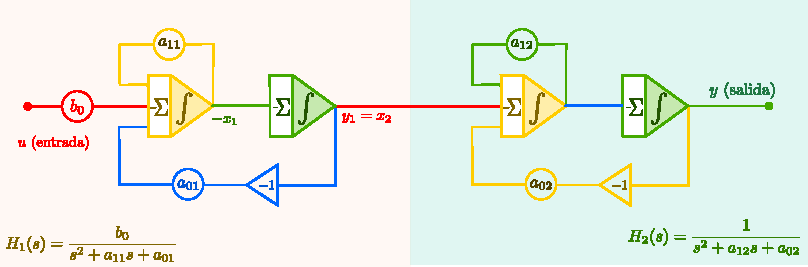
\includegraphics[width=1\textwidth]{figuras/filtrocomp}
	\caption{Diagrama de computación analógica del filtro de la ecuación \eqref{equ:filchebgen}.}
	\label{fig:filtrocomp}
\end{figure}

Para mostrar que esa es implementación analógica consideremos las ecuaciones de estado de $H_1(s)$, dadas por: 

\begin{align}
	\dot{x_1}&= -a_{11}\,x_1 - a_{01} x_2 + b_0\,u\nonumber\\
	\dot{x_2}&= x_1\nonumber\\
	y_1&=x_2
\end{align}
Note que justamente el diagrama de computación analógica de la izquierda corresponde con esta descripción de estado (teniendo en cuenta que los integradores son inversores). De forma similar construimos $H_2(s)$.


\subsection{Pasos de implementación en el \tt{THAT}}

\begin{enumerate}[label=\alph*)]
\item ``Resetee el \that'', es decir, retire todos los conectores, incluido el RCA. Ponga el \that en modo  \tt{OFF}.

\newpage
\item  Conecte el generador de ondas a la entrada \tt{U} como se muestra en la figura~\ref{fig:generador}, usando el adaptador BNC-RCA provisto.
 %
\begin{figure}[h!]
	\centering
	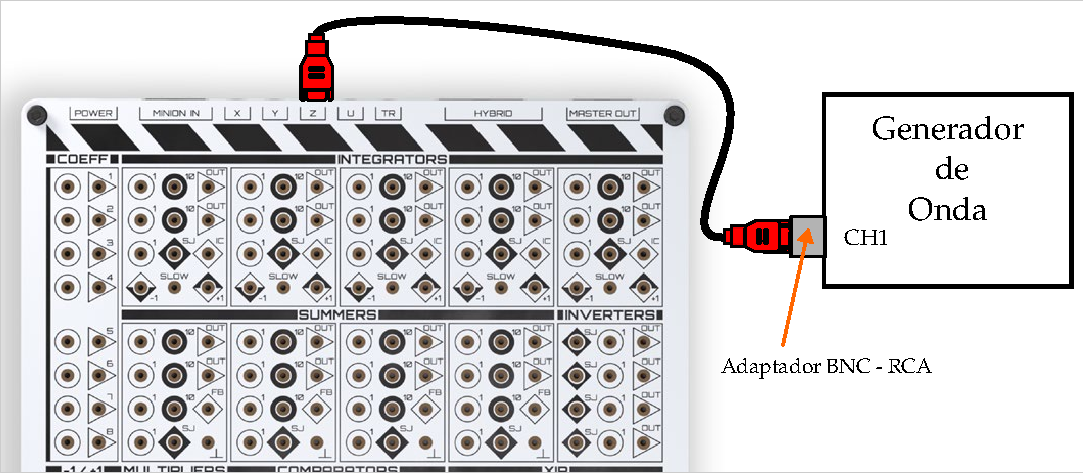
\includegraphics[width=0.7\textwidth]{figuras/generador}
	\caption{Conexión del generador de ondas.}
	\label{fig:generador}
\end{figure}
\item Identifique claramente cada uno de los componentes del diagrama de la figura~\ref{fig:filtrothat}.
%
\begin{figure}[h!]
	\centering
	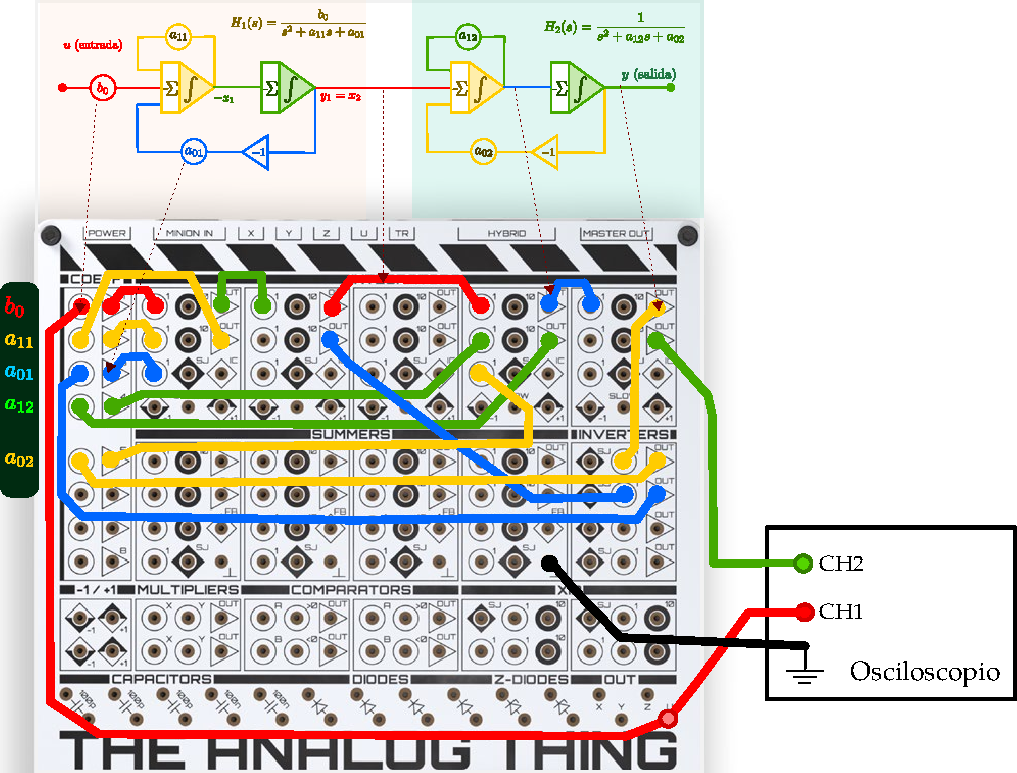
\includegraphics[width=1\textwidth]{figuras/filtrothat}
	\caption{Implementación del filtro en el \that.}
	\label{fig:filtrothat}
\end{figure}

Note que los coeficientes de las funciones de transferencia están asociados con las controles \tt{COEFF} del \that. Note que el cable rojo se usa para la onda de entrada y para la conexión entre las dos secciones.

\item  Implementar cuidadosamente el diagrama de computador analógico de la figura~\ref{fig:filtrothat}. Note que no es necesario (ni deseable) conectar la tierra del canal 2.

\item Acceda \href{https://colab.research.google.com/drive/1FAwNfmSHj2Xydje-8FpgHDbYV_laZE4f?usp=sharing}{a este colab} y corra la primera celda que diseña el filtro. Ponga el \that en modo \tt{COEFF} y ajuste cuidadosamente cada uno de los coeficientes del filtro. No se preocupe demasiado por la última cifra significativa, aunque el \that permite ajustarla con precisión mediante toques suaves al potenciómetro respectivo.

\item Ajuste el generador de onda con una señal sinusoidal de $50\,\text{Hz}$ y una tensión de $10\,\text{V}_{pp}$ ($5\text{V}_{p}$). Sincronice adecuadamente los canales del osciloscopio.

\item Ponga el \that en modo \tt{OP} (modo de operación continua, sin reseteo de integradores).
\item El filtro está diseñado para  $100\,\text{Hz}$. Suba y baje la frecuencia por encima y debajo de $100$ Hz para ``percibir''  el efecto del filtro.
\item Mida la atenuación en dB del filtro en las frecuencias de $50,100,150$ y $210\,$Hz. Compare con la atenuación provista en el diseño que aparece en el cálculo de la ultima celda \href{https://colab.research.google.com/drive/1FAwNfmSHj2Xydje-8FpgHDbYV_laZE4f?usp=sharing}{del colab.}

\item Ajuste el generador de onda en modo \tt{SWEEP} con frecuencia inicial de $10\,$Hz y una frecuencia final de $200\,$Hz. Ajuste el \tt{SWEEP TIME} en un segundo. Ajuste la escala del osciloscopio para ver la respuesta en frecuencia del filtro. Verifique que la frecuencia de corte es 100 Hz, mediante la escala de tiempo en el osciloscopio. 
 
\end{enumerate}

\newpage
\subsection{Rediseño del filtro para 200 Hz}

Ahora vamos a rediseñar el filtro para una frecuencia de 200Hz.
\begin{enumerate}[label=\alph*)]
\item Por medio del  \href{https://colab.research.google.com/drive/1FAwNfmSHj2Xydje-8FpgHDbYV_laZE4f?usp=sharing}{colab} rediseñe el filtro para una frecuencia de 200Hz.


\item Ajuste los coeficientes respectivos. 

\subsubsection*{\label{sec:coefmay} Nota Coeficientes mayores a la unidad}
Es posible que algunos den valores mayores a 1. En ese caso podemos usar el modo de multiplicación $\times 10$ presente en las entradas de cada integrador. Por ejemplo, supongamos que el coeficiente $a_{11}=2.25$.
%
\begin{figure}[h!]
	\centering
	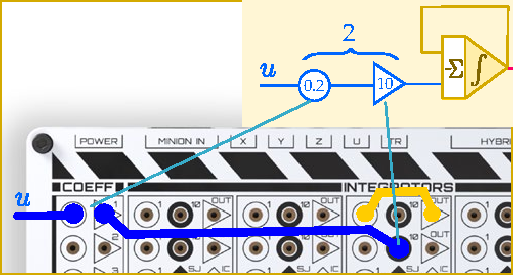
\includegraphics[width=.8\textwidth]{figuras/ejemplo}
	\caption{Implementación de un coeficiente mayor a la unidad.}
	\label{fig:ejemplo}
\end{figure}

Como se ilustra en la figura~\ref{fig:ejemplo}, podemos implementar este coeficiente en el \that si ajustamos $0.225$ en el potenciometro correspondiente y al mismo tiempo lo introducimos multiplicado por 10 en el integrador. Así, el valor equivalente que estamos colocando a la entrada del integrador es:
\[a_{11}=10 \times 0.225=2.25\]

\item Verifique que la nueva frecuencia de corte es $200$ Hz, variando apropiadamente la frecuencia del generador.

\item Ajuste una onda \tt{SWEEP} y 	verifique el funcionamiento del filtro. 
\end{enumerate}

\newpage

\section{Estabilidad de un sistema realimentado y test de estabilidad de Routh- Hurwitz}

En esta última sección vamos a analizar la estabilidad del sistema realimentado de la figura~\ref{fig:realimentado}:
%
\begin{figure}[h!]
	\centering
	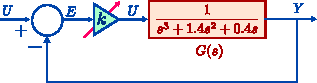
\includegraphics[width=.65\textwidth]{figuras/realimentado}
	\caption{Implementación de un coeficiente mayor a la unidad.}
	\label{fig:realimentado}
\end{figure}

Este sistema tiene función de transferencia de lazo cerrado $H_r(s)$, dada por:
\begin{align}
H_r(s) = \dfrac{Y(s)}{U(s)} &= \dfrac{kG(s)}{1+kG(s)}\nonumber\\
	   &= \dfrac{k}{s^3+1.4s^2+0.4s+k}
	   \label{equ:realimentado}
\end{align}



Queremos analizar experimentalmente la estabilidad de $H_r(s)$  para variaciones del parámetro $k$ en que $0 \leq k \leq 1$, usando el \that

\newpage
\subsection{Implementación}

Note que la función $G(s)$ en el lazo realimentado la podemos expresar como:

\begin{align}
	G(s)&=G_1(s) \times G_2(s) \times G_3(s) \nonumber\\
	&=\dfrac{1}{s+1} \times \dfrac{1}{s+0.4} \times \dfrac{1}{s}.
\end{align}

 Y cada bloque de primer orden lo podemos realizar como se ilustra en la figura~\ref{fig:analoghurwitz}
 %
\begin{figure}[h!]
	\centering
	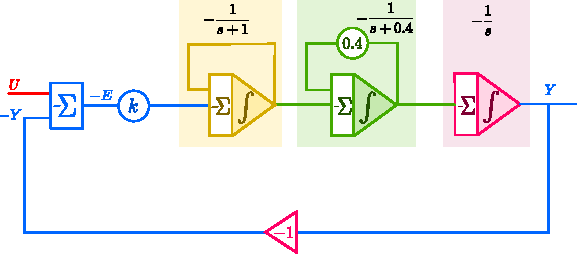
\includegraphics[width=.9\textwidth]{figuras/analoghurwitz}
	\caption{Implementación de computador analógico.}
	\label{fig:analoghurwitz}
\end{figure}


\subsection{Pasos de implementación}

\begin{enumerate}[label=\alph*)]
		
	\item Discuta con su compañero, porque los bloques en color de la figura~\ref{fig:analoghurwitz} implementan a $G_1$, $G_2$ y $G_3$.
	
	\item Desconecte todos los cables del \that, incluyendo el conector RCA y el generador de onda.
	
	\item Realice nuevamente el generador de onda del \that~ de  la sección~\ref{sec:cuadrada} 
	
	\item Implemente cuidadosamente en el \that~ el diagrama de la figura \ref{fig:analoghurwitz}. Use los bloques apropiados.
	\item Conecte el canal 1 y el canal 2 a la entrada $U$ y la salida $Y$ del sistema como en la figura~\ref{fig:analog2orderthat}.
	
	\item Ponga el \tt{THAT} en modo \tt{REPF}.
	
	\item Varie el coeficiente correspondiente a $k$ y determine por la respuesta percibida en el osciloscopio, el punto en que el sistema cambia de estable a inestable. Registre este valor pasando el \tt{THAT} al modo \tt{COEFF}.
	
	\item Use el criterio de Routh - Hurwitz  para obtener matematicamente el rango de estabilidad del sistema realimentado de la ecuación~\eqref{equ:realimentado} (puede usar gemini u otra). Compare con lo obtenido experimentalmente.
\end{enumerate}

\end{document}
